\documentclass[a4paper,10pt]{report}
\usepackage{geometry} % change page margins/layout
%\usepackage[ngerman]{babel} % document Germanisation
\usepackage[utf8]{inputenc} % German umlauts
\usepackage[T1]{fontenc} % accented language characters
\usepackage{bm} % better bold symbols
\usepackage{graphicx} % better image handling
\graphicspath{ {images/} }
\usepackage{wrapfig} % text wrap around images
\usepackage{subcaption} % subfigures
\usepackage[section]{placeins} % float barriers
\usepackage{booktabs} % better looking tables
\usepackage{makecell} % multi-rows in table cells
\usepackage[shortlabels]{enumitem} % better lists
\usepackage{amsmath,mathtools,amssymb} % math typesetting/symbols
\usepackage{nicefrac} % in-line looking fractions
\usepackage[version=4]{mhchem} % chemical elements
\usepackage[locale = US, 
			separate-uncertainty,
			exponent-product = \cdot,
			output-product = \cdot,
			per-mode=reciprocal]{siunitx} % easy uncertainties
\usepackage[hyphens]{url} % allows for URL breaks
\usepackage[colorlinks=true,linkcolor=black,
			urlcolor=blue,citecolor=black]{hyperref} % URL links
\usepackage[english]{cleveref} % better referencing
\usepackage{titlesec} % title section formatting
\titleformat{\chapter}{\bfseries\LARGE}{\thechapter~}{0em}{}
\usepackage[autostyle]{csquotes} % better quotes

\usepackage{xcolor}
\usepackage{listings} % for code
\definecolor{codegreen}{rgb}{0,0.6,0}
\definecolor{codegray}{rgb}{0.5,0.5,0.5}
\definecolor{codepurple}{rgb}{0.58,0,0.82}
\definecolor{backcolour}{rgb}{0.95,0.95,0.92}
\lstdefinestyle{mystyle}{
	backgroundcolor=\color{backcolour},   
	commentstyle=\color{codegreen},
	keywordstyle=\color{magenta},
	numberstyle=\tiny\color{codegray},
	stringstyle=\color{codepurple},
	basicstyle=\ttfamily\scriptsize,
	breakatwhitespace=false,         
	breaklines=true,                 
	captionpos=b,                    
	keepspaces=true,                 
	numbers=left,                    
	numbersep=5pt,                  
	showspaces=false,                
	showstringspaces=false,
	showtabs=false,                  
	tabsize=2
}
\lstset{style=mystyle}

% DARK-MODE on PDF reader
\usepackage{xcolor}
\pagecolor[HTML]{1f1f1f} % dark color
\color[HTML]{c7c7c7} % light color

\setcounter{tocdepth}{2}
%------------------------------------------------------------------


\begin{document}


\title{
	\vspace{2cm}
	{\LARGE Electric Vehicles in Energy Communities:}\\
	{\Large Investigating the Distribution Grid Hosting Capacity} \\[2cm]
	{\large Albert Ludwig University of Freiburg}
}
\author{
	\Large Daniil Aktanka
}
\date{
	\normalsize \today
}
\maketitle
\thispagestyle{empty}


\pagenumbering{roman}
\chapter*{Abstract}
\addcontentsline{toc}{chapter}{Abstract}

The global trend towards electric vehicle (EV) adoption poses numerous challenges for the traditional electric grid operations and infrastructure. This paper examines the stability of low-voltage European grids in the context of EV integration. For this purpose, a power flow analysis is performed based on historical data of residential load profiles. A critical case scenario is used for computing the hosting capacity's upper and lower limits. The results show $\approx 11\,\%$ and $\approx 22\,\%$ grid hosting capacities for worst and best case scenarios respectively. The coordination of individual households within the grid is explored via a newly proposed spacio-temporal charging algorithm for a basic energy community.  A comparison between a random charging pattern and a semi-coordinated energy community charging pattern is made based on a set of timeseries simulations. The results suggest that the energy community algorithm is $\approx 30\,\%$ more effective than the random case; the proposed energy community model is suggested as an intermediary solution for a transition towards future smart grids.


\listoftables
\addcontentsline{toc}{chapter}{List of tables}
\cleardoublepage

\listoffigures
\addcontentsline{toc}{chapter}{List of figures}
\cleardoublepage

\tableofcontents\cleardoublepage

\pagenumbering{arabic}


\chapter{Introduction}
Electrification of transportation represents a major role in a move towards a sustainable future of energy systems. It brings about a number of interdisciplinary challenges, requiring simultaneous coordination from multiple fields of study. This paper aims to address one of these components from the perspective of the power distribution network---namely, the hosting capacity limitations of the electric grid.

\begin{figure}[htpb]
	\centering
	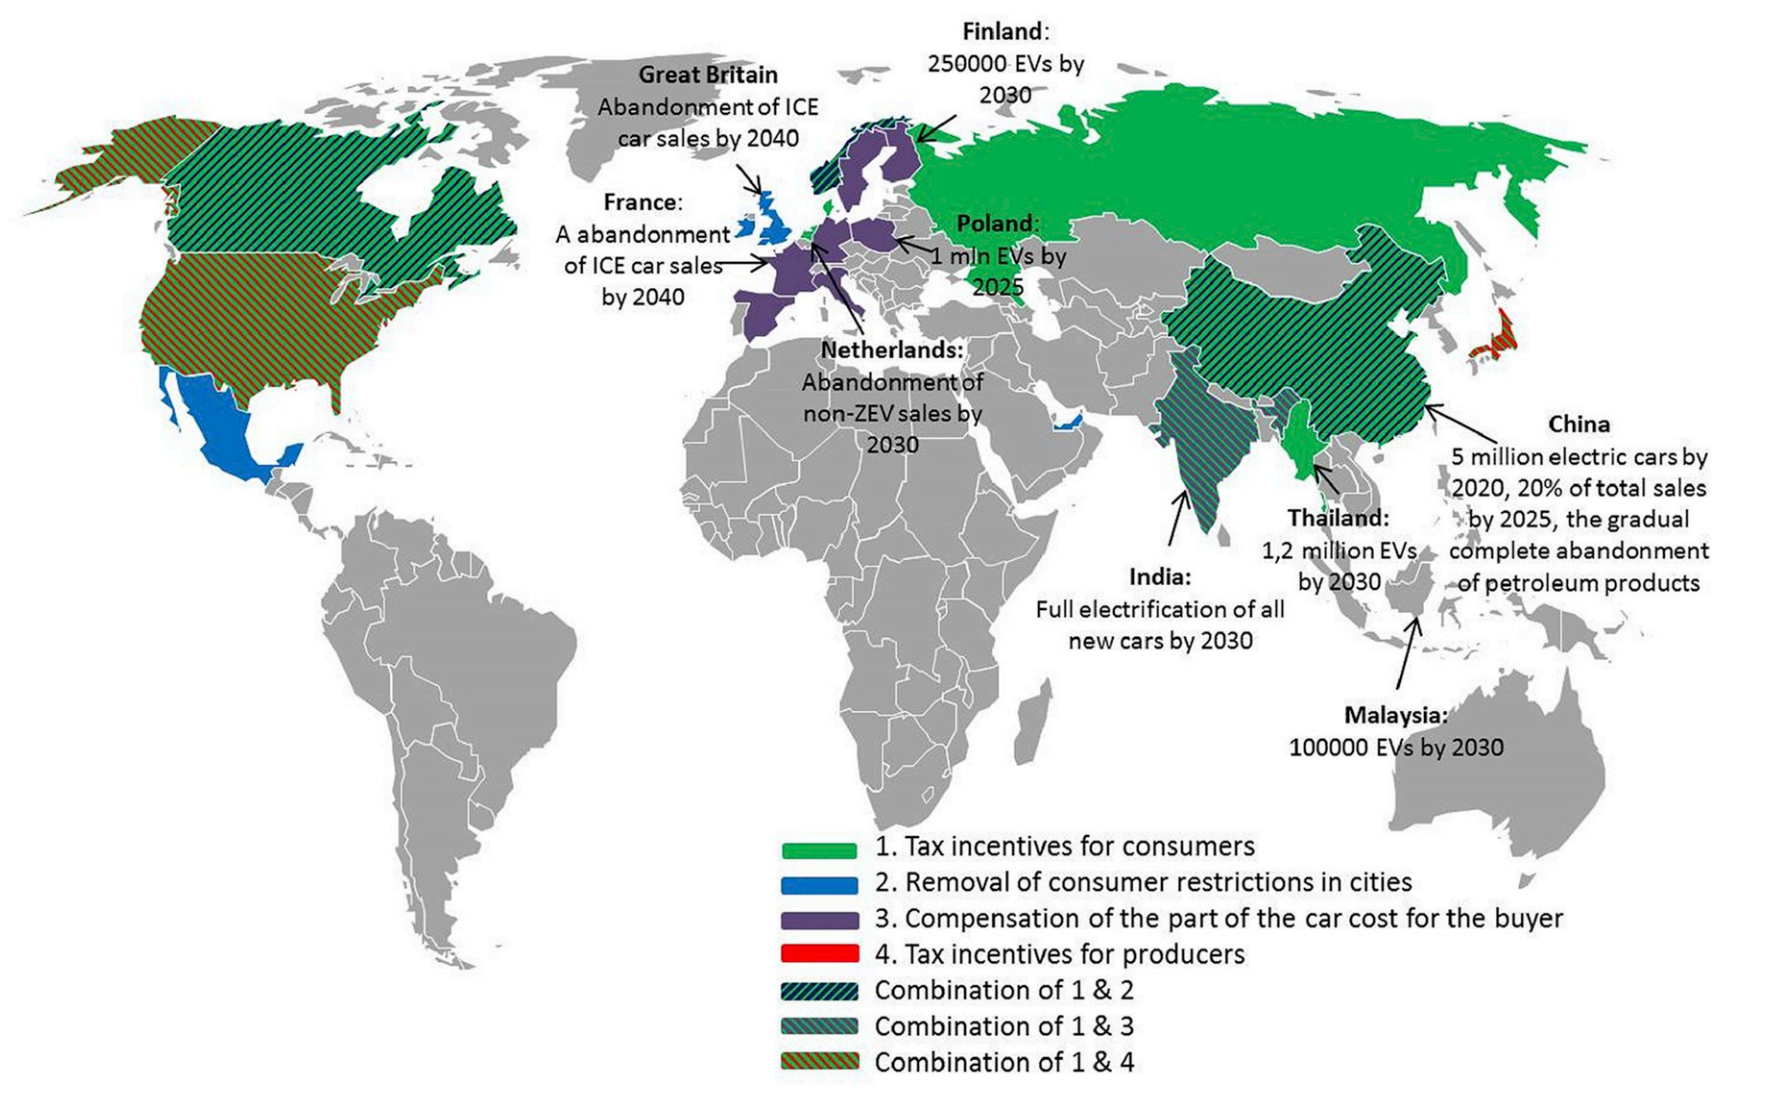
\includegraphics[width=\linewidth]{ev_state_support_mech}
	\caption[EV state support and goals]{Electric vehicles state support mechanisms and national goals across the world. \cite{Kapustin2020}.}
	\label{ev_state_support_mech}
\end{figure}

The transition from internal combustion engine (ICE) vehicles to electric vehicles (EVs) has entered world-wide adoption. A large portion of the western world has already set hard targets in order to facilitate this transition, ranging from tax incentives to outright abandonment of ICE car sales within the next 20 years (see \cref{ev_state_support_mech}). While the EV technology has made tremendous advancements over the past several decades---especially in terms of mobility range---this alone may not be enough for complete integration of EVs. Full-scale transition towards EV adoption would require the underlying infrastructure to be able to support charging, discharging (Vehicle-to-Grid) and coordinated management of EVs. However, contrary to the rapid development of EV technology, the electric grid remained relatively unchanged since the years of its early inception. The coveted transition towards the smart grid is mostly not feasible as a single-step on a large scale, which begs the question of how well does the existing system accommodate the transition towards EV integration.

This paper aims to investigate this question from multiple angles. The main premise is a simple substitution of ICE vehicles for EVs in the context of the current grid under a multitude of assumptions. The scope of this study is limited to the low-voltage grid, to which all of the EV charging is hypothetically constrained. Furthermore, no public charging stations were considered in this study. Despite their growing popularity, the goal of this paper was to investigate the minimum investment conditions for near-future EV charging scenarios; as such, only residential home chargers were considered.

The main method employed in this paper's study is a power flow analysis using randomized historical load profiles. Hereby the biggest block of information processing was arguably the data analysis, the details of which will be described first. Next, the concepts of various charging strategies will be introduced in a form of three scenarios: critical case, random time and energy community. Finally, the results will be presented in 2 parts: hosting capacity evaluation and the comparison between random and energy community scenarios. Additionally, suggested improvements will be provided for multiple areas of this paper.


\chapter{Related Work}
\section{Literature review}\label{section_literature_review}
The inspirational starting point for this thesis was the paper "Electric vehicles standards, charging infrastructure, and impact on grid integration: A technological review" by H.S. Das et al. \cite{Das2020}. It provides a comprehensive overview of the current EV status and the challenges of EV integration across multiple organizational fields. Notably, it classifies EV charging control strategies across different attributes, as seen in \cref{control_strats_charging}. Hereby the concept of coordinated vs uncoordinated charging strategies became one of the main focal points for this thesis paper, leading to the introduction of the semi-coordinated charging method. Further points of interest in H.S. Das's paper include the distinction between centralized and decentralized control architectures, as seen in \cref{centralized_vs_decentr_ctrl}. The researchers claim that decentralized/distributed mechanisms are superior in terms of computational complexity, real-time implementation and offer more user convenience. In a similar fashion, the paper "Integration of electric vehicles and management in the internet of energy" by K. Mahmud et al. discusses the future grid and the essentials of adaptive charging infrastructure for EV integration, noting the importance of coordinated EV management \cite{Mahmud2018}.

\begin{figure}[htpb]
	\centering
	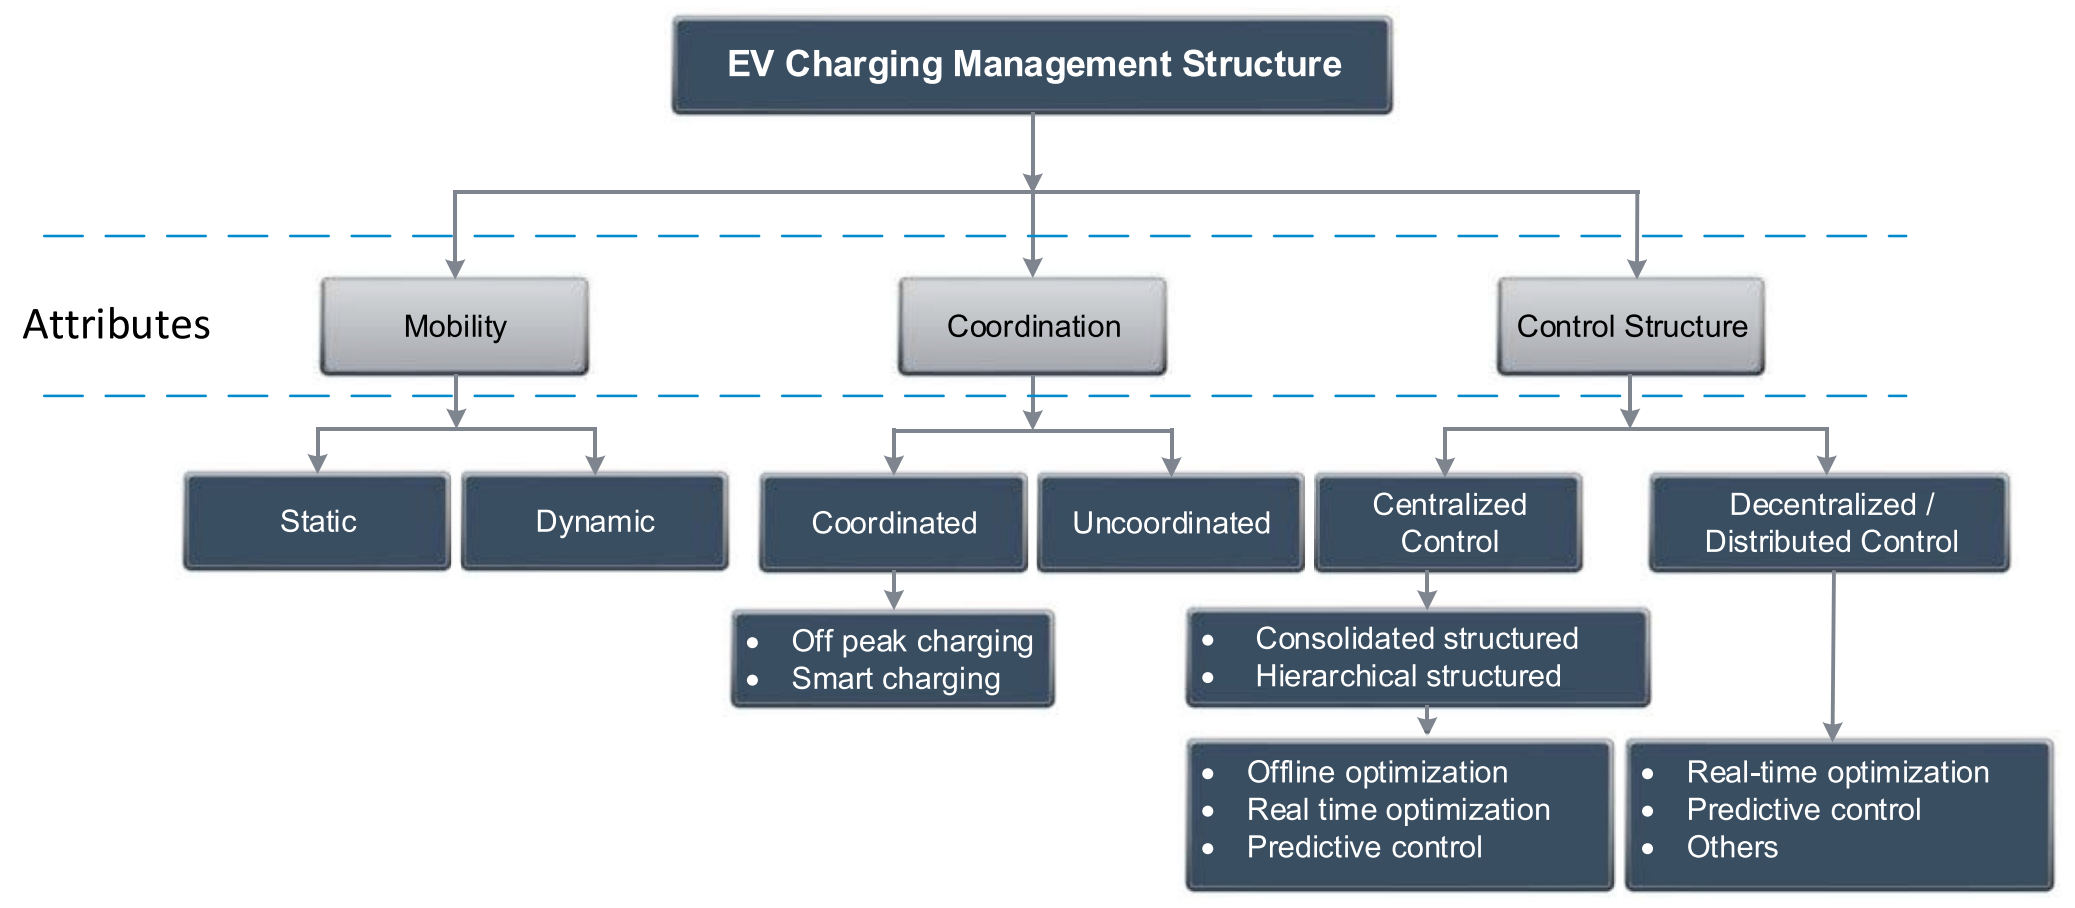
\includegraphics[width=\linewidth]{control_strats_charging}
	\caption[]{Classification of control strategies used in EV charging system \cite{Das2020}.}
	\label{control_strats_charging}
\end{figure}

\begin{figure}[htpb]
	\centering
	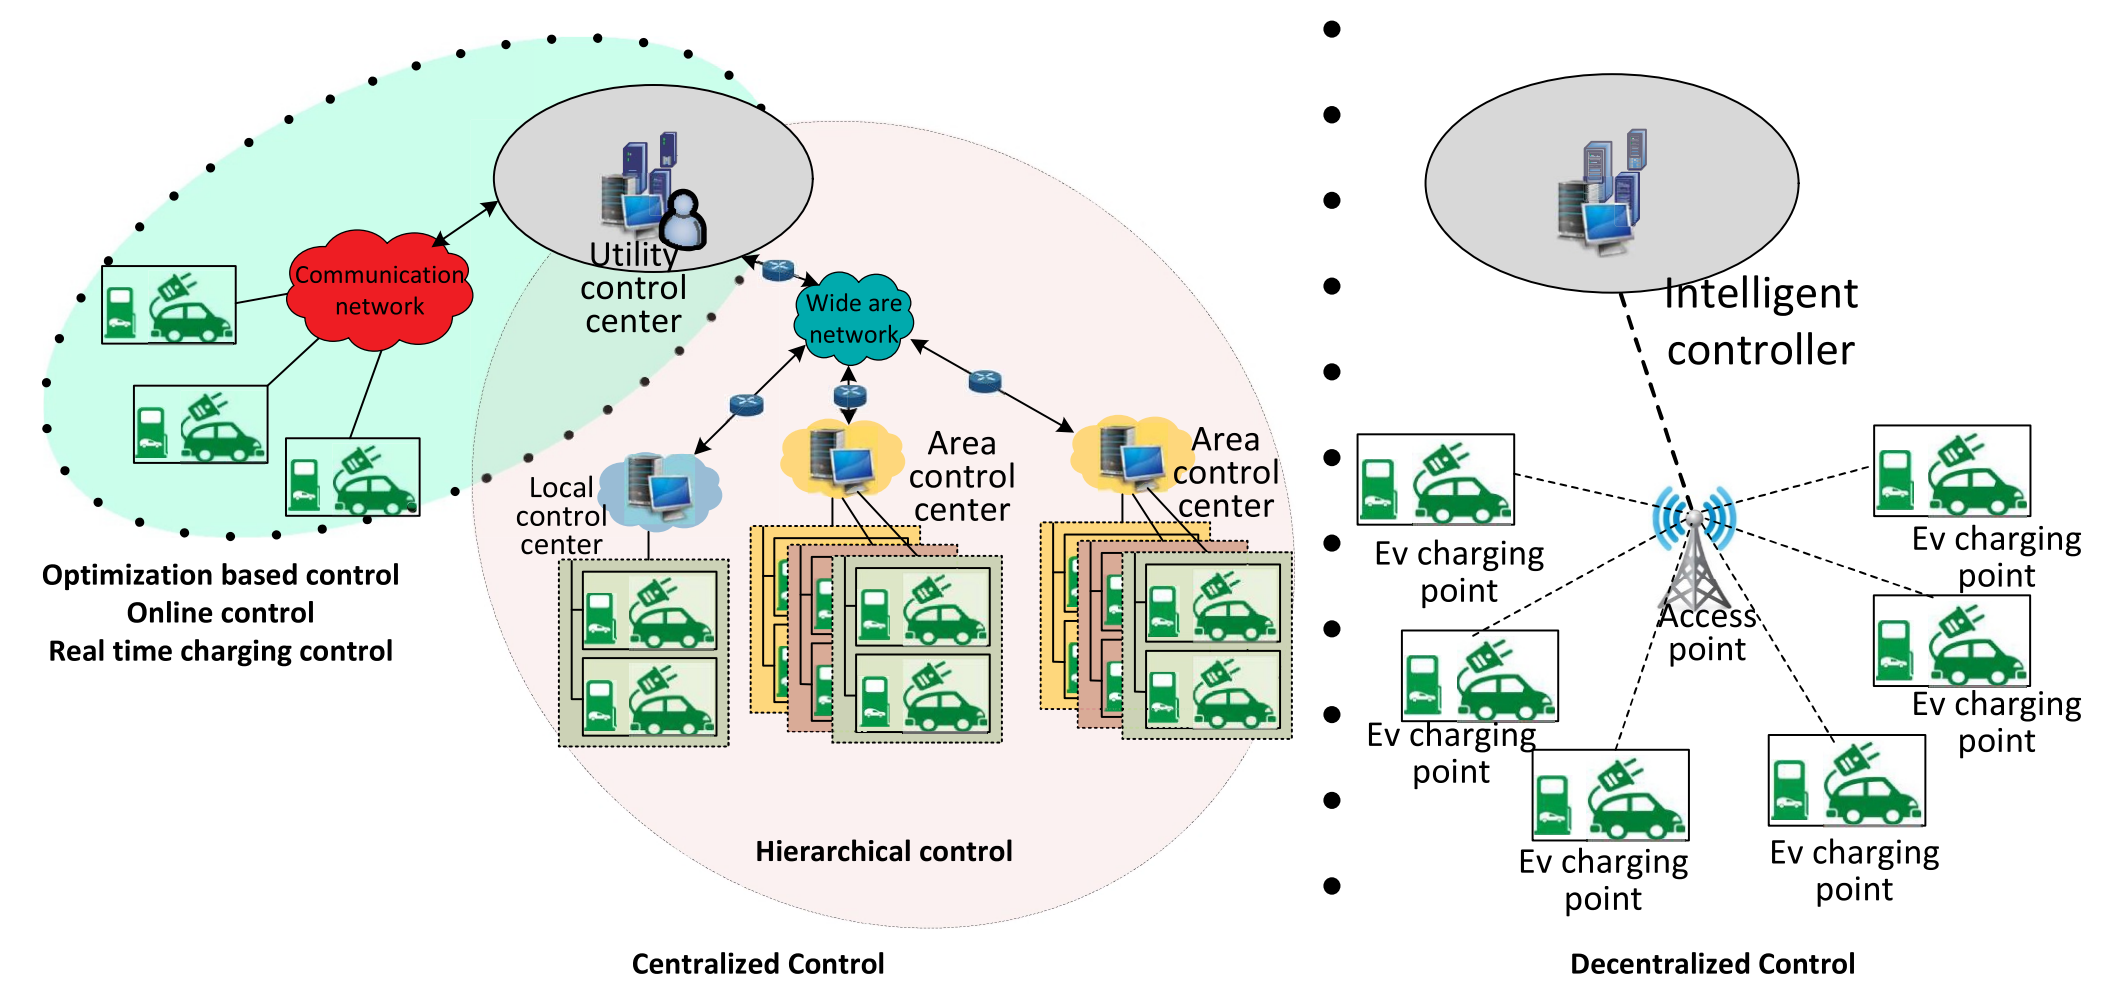
\includegraphics[width=\linewidth]{centralized_vs_decentr_ctrl}
	\caption[Centralized and decentralized control architecture]{Centralized and decentralized control architecture of EV charging system \cite{Das2020}.}
	\label{centralized_vs_decentr_ctrl}
\end{figure}

A more advanced variation of this paper's method can be found in an IEEE Access article "Uncertainty-Aware Computational Tools for Power Distribution Networks Including Electrical Vehicle Charging and Load Profiles" by Giambattista Gruosso et al. \cite{Gruosso2019}. It describes an efficient, uncertainty-aware load flow analysis reliant on generalized Polynomial Chaos and Stochastic testing methods. The authors use historical load profiles to simulate variation in both residential loads and EV charging profiles, which was additionally compared against a Monte Carlo simulation. Similarly to this thesis, an example network of choice was the European Low-Voltage Test Feeder, whereby all of the loads were assumed to be single phase. The result was a technique able to account for real data-based load profiles for network quality assessment.

For the computation of distribution grid hosting capacity, consider the paper "Optimization-based distribution grid hosting capacity calculations" by Mansoor Alturki et al. \cite{Alturki2018}. The authors propose an optimization-based method for determining the hosting capacity using linear power flow equations. Unlike traditional nonlinear models, the proposed method does not rely on iteration in order to find a near-optimal hosting capacity solution. The obtained solution at operating point provides access to both active and reactive power flow information, additionally accounting for seasonal load variations. A more common, iterative approach---such as the one used in this paper---can be found in "EV Hosting Capacity Analysis on Distribution Grids" by Priti Paudyal et al. \cite{PritiPaudyal2021}.

The paper "Applying responsible algorithm design to neighbourhood-scale batteries in Australia" by H. Ransan-Cooper et al. is an interdisciplinary study that examines the systemic concerns to design and operation of energy algorithms. The study focused on comparing 6  different metrics used for algorithm design, whereby the algorithm of interest is the timer algorithm. "The timer algorithm is designed to challenge assumptions in techno-economic optimization by explicitly forgoing economic or environmental optimization to instead optimize for explainability as a response to citizen concerns about a lack of transparency in the energy system" \cite{RansanCooper2021}. Interestingly, the timer algorithm employed the same night window as the one used in this paper. The researchers claim that "it is possible that non-‘optimal’ timer algorithms may meet public needs because they relieve concerns about complexity and a lack of transparency" \cite{RansanCooper2021}. This statement directly supports the motivation behind this paper's energy community algorithm.

The next section will summarize the basics of the power flow analysis and nonlinear models.

\newpage
\section{Power flow analysis}
Power flow (or load flow) study is a numerical analysis of the flow of electric power in a network. Its objective is to calculate the bus voltages---consisting of magnitudes and angles---given the network conditions defined by loads, generation and other variables. The busses are classified into 3 types: load, generation and slack. Load (or PQ) busses have no generators connected to them. Conversely, all busses with at least one generator connected to them are called generator (or PV) buses, with one arbitrary exception---the slack bus. Also known as the swing or reference bus, the slack bus is used to compensate for system losses by either emitting or absorbing active and reactive power within the system. For a system consisting of $n$ buses and $g$ generators, there are $2(n-1)-(g-1)$ unknowns. In order to solve for these unknowns, a special admittance matrix is used to construct real and reactive power balance equations. This results in a system of nonlinear equations which can be solved in a variety of methods. The most common method is the Newton-Raphson method.

The Newton-Raphson technique is a method of successive approximation based on the Taylor's expansion approximation used to solve $f(x)=c$. In the context of power flow problems, the unknown variables $x$ are: voltage magnitude at load busses ($\lvert V_i\rvert$), angles at load busses ($\angle\delta_i$) and voltage angles at regulated buses ($\delta_i$). The specified quantities $c$ are both the net scheduled (known) injected real power ($P_i^{sch}$) and the net scheduled injected reactive power ($jQ_i^{sch}$).

The iterative values of real power are calculated using:
\begin{equation}
	P_i^{[k+1]}=\sum^{n}_{j=1}\lvert V_i\rvert^{[k]}\lvert V_j\rvert^{[k \text{ or } k+1]}\lvert Y_{ij}\rvert\cos\Bigl(\Theta_{ij}-\delta_i^{[k]}+\delta_j^{[k]}\Bigr)
\end{equation}

The iterative values of reactive power are calculated as:
\begin{equation}
	Q_i^{[k+1]}=-\sum^{n}_{j=1}\lvert V_i\rvert^{[k]}\lvert V_j\rvert^{[k \text{ or } k+1]}\lvert Y_{ij}\rvert\sin\Bigl(\Theta_{ij}-\delta_i^{[k]}+\delta_j^{[k]}\Bigr)
\end{equation}

whereby $Y$ is a symmetrical admittance matrix, consisting of admittance values of both lines and busses. The Newton-Raphson power flow formulation can be solved using the following \cref{nr_form}. See "Computational Models in Engineering" for more details \cite{Albadi2020}.
\begin{equation}\label{nr_form}
	\begin{bmatrix}
		\Delta P_i^{[k]}\\
		\Delta Q_t^{[k]}
	\end{bmatrix}
	=
	\underbrace{
		\begin{bmatrix}
			\frac{\partial P_i}{\partial \delta_i}^{[k]} & \frac{\partial P_i}{\partial \lvert V_i \rvert}^{[k]}\\
			\frac{\partial Q^i}{\partial \delta_i}^{[k]} & \frac{\partial Q^i}{\partial \lvert V_i \rvert}^{[k]}
		\end{bmatrix}
	}_{\llap{\small Jacobian matrix\:}
		f'\,=\,
		\begin{bmatrix}
			J_{P\delta} & J_{P\lvert V\rvert}\\
			J_{Q\delta} & J_{Q\lvert V\rvert}
		\end{bmatrix}
	}
	\begin{bmatrix}
		\Delta\delta_i^{[k]}\\
		\Delta\lvert V_i \rvert^{[k]}
	\end{bmatrix}
\end{equation}

In this paper, we will be using the standard Newton-Raphson method. Some of the other power flow analysis methods include the Gauss-Siedel method, the fast-decoupled-load-flow method, the backward-forward sweep (BFS) method as well as the DC power flow technique. 


\chapter{Goal and Method}
\section{Approach}\label{section_approach}
The goal of this thesis was to investigate the distribution grid hosting capacity of electric vehicles and the effect the involvement of energy communities can have on it. Over the span of roughly two months, the method presented in this paper went through countless iterations in terms of functionality as well as network application (down to the last two weeks before deadline). The original testing models were performed on a simple test network with arbitrary values (see \cref{test_network}). These tests were done in order to get a feel for the chosen software tools and to better understand their potential real world application and the required scope of work.

\begin{figure}[htpb]
	\centering
	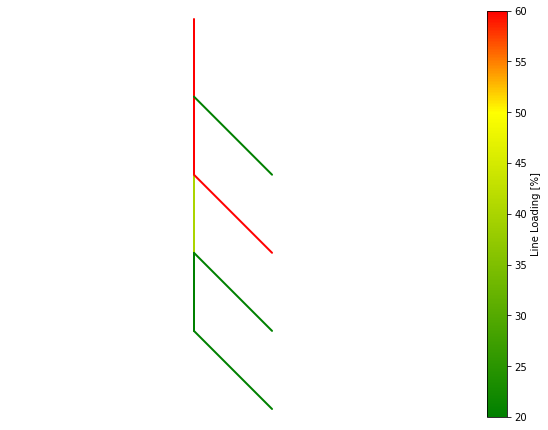
\includegraphics[width=0.46\linewidth]{test_network}
	\caption[Example power flow network with generic coordinates]{An example power flow calculation plot with line loading results. Here, one static generator is active out of four. The example network has generic coordinates instead of geographical, as seen in the rest of the plots in this paper.}
	\label{test_network}
\end{figure}

Early on, it was decided to incorporate real-world data as a basis of the simulation. Arguably the best (at the time of writing) data platform for this application is Open Power System Data---more specifically, the contributed household data package. It contains measured timeseries data for various households and businesses relevant for low-voltage power system modeling. In terms of geographical scope, it incorporates data from 11 households in Konstanz, southern Germany, as part of the CoSSMic project for the optimization of energy systems in smart cities. The gathered data is quite expansive, spanning a time range of over 4 years with a resolution of up to 1 minute measurements, even tracking single-device consumption. Cumulative energy measurements accounted for data gaps from communication problems and "all data gaps are either interpolated linearly, or filled with data of prior days" \cite{OpenPowerSystemData}, though no further detail is provided in this regard. Overall, this was the perfect fit for this paper's simulation aimed at a standard European low-voltage grid of a residential area.

Using and incorporating the Open Power System Data household dataset proved to be quite a challenge on its own. Details regarding final data analysis are described in \cref{section_data_processing}. Once the data was processed and loaded into the network for further computations, the question became how to formulate and subsequently evaluate simulation scenarios. Hereby, the number of variables to take into account can practically be expanded far beyond the scope of the paper. For instance, an alternative tool considered for the simulation of load data was the LoadProfileGenerator (LPG), which is a highly-customizable tool for modeling residential energy consumption. LPG performs complete behavior simulation of a household residents in order to generate load curves. To that extent, it would have been possible to take said curves and implement them into our network case, while investigating individual households' behaviors across a community of like-minded, cooperative individuals. However, this was deemed far too comprehensive given the time constraints, but also not as potentially insightful.

Additionally, in order to make best use of the historical data, it was decided to perform timeseries iteration of power flows. In a sense, this provides a similar advantage to LPG's functionality by mimicking random human behavior over time, only with no unnecessary explanations behind it. The main idea became to sample a random historical load profile per household and to consider when/how an EV charger could optimally function in time. While this may be a relatively simple question to answer for a single household---given the residents' preferences and habits, it's merely a load optimization problem---the main issue lies with multiple parties involved. In turn, those parties are connected on a network in different ways, bringing topology into account. Thus, time and space both dictate the conditions for a given network.

Eventually, the abstract example network got superseded by the benchmark European Low Voltage Test Feeder (from hereon: test feeder) (see \cref{EU_LV_test_feeder}). Three scenarios were chosen for evaluation: critical case, random charging, semi-coordinated charging. The critical case is used for hosting capacity evaluation of our simulation for singular time points, whereas the two other scenarios demonstrate time-dependent charging behavior models. Detailed explanation for this approach is given in \cref{section_network_application}. From hereon, EV home charging stations will be referred to as (negative) static generators in the context of power modeling. %

\begin{figure}[htpb]
	\centering
	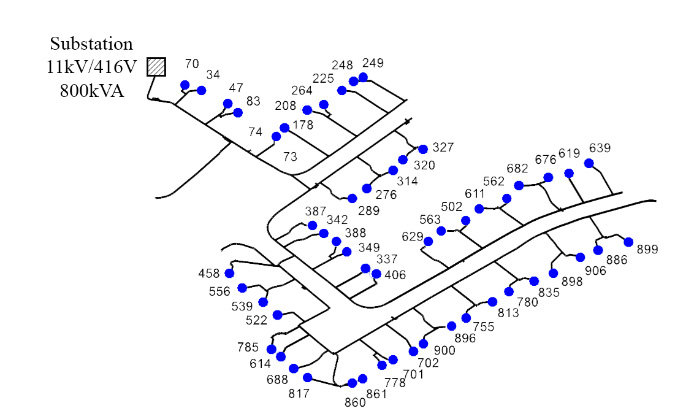
\includegraphics[width=0.6\linewidth]{EU_LV_test_feeder}
	\caption[European Low Voltage Test Feeder layout]{European Low Voltage Test Feeder network illustration. The blue dots are the active busses, representing households \cite{Nousdilis2017}.}
	\label{EU_LV_test_feeder}
\end{figure}

The next section will describe the functionality of custom python classes. For more details, consult the source code on GitHub at: \url{https://github.com/akthonka/EV_energy_comm} .

\newpage
\section{Data processing}\label{section_data_processing}
Given the scope of the project, the idea was to create a system flexible enough for iterative data manipulation and ideally one that would support multiple network types. The project was written entirely in python due to language simplicity as well as availability of advanced libraries. Data handling was done using the \texttt{pandas} library, whereas the network simulation was performed using the \texttt{pandapower} toolbox library.

For the sake of clarity, most of the code was split between a python class file and jupyter notebooks. For early testing and code prototyping, jupyter notebooks are sufficient but they quickly lose readability as the code complexity grows. The general methodology was therefore to write core functions in jupyter to then integrate them into an external python class file. The resultant python class file consists of two classes: one for handling data processing and another for operations based on the \texttt{pandapower} library. Common input settings (for instance, the time window) are saved as class variables, such that only the most top-level functions are called in jupyter.

\subsection{DataAction class}
The following information describes the code of the python class responsible for core data processing. While the general methodology is applicable to any dataset, these functions are tailored specifically to the household dataset (\texttt{household\_data\_1min\_singleindex\_filtered.csv}) and will be described as such. Additionally, the functions mentioned here target the test feeder network as our simulation case but can be adapted for any network, with several caveats mentioned later. The following paragraphs serve to summarize the operation of one or more functions based on their application.

\paragraph{Data import and segmenting:} The raw dataset is imported as a dataframe without additional options. Dropping the rest, we keep only 3 columns: \texttt{DE\_KN\_residential1\_grid\_import}, \texttt{DE\_KN\_residential2\_grid\_import} and \texttt{utc\_timestamp}. Since we will be performing conditional time-based operations, we set the timestamp column as index for ease of use. While it is possible to front-load a lot of data processing functions at this step---such as parsing datetimes---it is not recommended due to unnecessary computation time. A better approach is to segment the data for piece-wise processing and function testing, whereby it would be possible to iterate computations over the entire dataset in the future. Therefore, we split the imported dataframe (of a little over a million data points) into a list of smaller dataframes (each 10000 data points long, with residual last dataframe being a bit smaller). If you are using class variables for storing the dataframe list, don't forget to clear it before each sampling run when performing bulk simulations (see \cref{subsection_additional}).

\paragraph{Datetime parsing function:} This function converts a segment of the imported data into a specific, time-indexed dataframe. First, we parse the datetime index, specifying the format as \texttt{"Year--Month--Day Hour:Minute:Second"}, after which we convert from UTC to Berlin time---the local time of the recorded dataset. While it is possible to import data with local time column \texttt{cet\_cest\_timestamp} without the need of conversion, it is not recommended for \texttt{pandas 1.4.3} since that will cause errors in datetime operations based on author's experience. Second, we take the difference between consecutive rows. This is done in order to obtain minute-wise energy changes, since the household dataset only tracks cumulative energy values. If we use the \texttt{pandas.diff()} function, we must also drop the resulting first row, since it's a NaN row.

\paragraph{Night profile functions:} This set of functions is fundamental for the simulation, as they are used to create a load profile for a single household. First, we must select a random dataframe segment with either of the two historical load profiles and parse it for datetime. The segment contains data on several days/nights, the dates of which we must identify. Then, for a random date, we must get the starting and ending datetimes for dataframe slicing. Knowing the starting time of our window---in our case, \texttt{18:00:00}---we need to create a datetime object for the chosen date, given the starting time. From said datetime (for example, \texttt{2015-08-16 18:00:00}) we add one day to the date and update the time with our morning value (getting \texttt{2015-08-17 06:00:00}). With these two datetimes, we can now slice the selected dataframe to obtain the required single house overnight load profile. Such datetime manipulations are very commonplace for this simulation.

\paragraph{Create loads and static generators:} This function creates the dataframes used for timeseries iteration---from hereon referred to as night dataframes. These hold the inputs for the network values, for both the loads as well as the static generators (sgens). Depending on the timeseries controller, it is important to create the night dataframes in a very specific way: the names and the indices of the network components will dictate the conventions. Unless you are writing your own controller, refer to your documentation for more details.

To create the night dataframes, first get a random night profile. This contains all the necessary time steps in the index, which is what we need; the load values can be set to zero. Then, generate a list of appropriate load names and form a dataframe using the time index. For the case of the test feeder network, the resulting night dataframes are 721 rows $\times$ 55 columns (minutes $\times$ number of profiles). Repeat for both loads and sgens night dataframes. It is recommended to save these as class variables, since we will be referencing them throughout the entire simulation, as well as for troubleshooting purposes. Finally, we convert our night loads to MW units via a simple conversion factor multiplication.

\paragraph{Random static generators:} These functions fill the night sgen dataframe at random times with a select sgen value. It's recommended to first reset the night dataframe by setting all sgen values to zero, otherwise location slicing may not overwrite the value. Getting a random set of starting and ending datetimes follows the same principle as described for night profile functions. It's important to keep track of zero-based indexing when calling random values from range. Additionally, in case of \texttt{pandapower}, the sgen sign needs to be set as negative in order to act as a separate static load that is an EV charger.

\paragraph{Energy community static generators:} These functions fill the night sgen dataframe iteratively and cyclically (see \cref{section_network_application} for motivation). This method consists of two parts. In the first part, the starting times for sgens are determined. The allowed time values are bound by the time window, and are dependent on the time step (charging time). To compute the list of starting charging times, begin with the evening time value and add the time step iteratively for the number of sgens present. In our case, we have 55 sgens and a time window of 12 hours; for a charging time of 1 hour, that would result in 12 starting charging times. If we only had 7 sgens in the same time conditions, we would have 7 starting charging times, etc. The next part concerns the starting time sgen cycle.

For best practice, set all night sgen values to zero before writing new ones. The following step was done using \texttt{cycle()} function from the \texttt{itertools} module in python. Beginning with the evening start time (see \cref{section_improvements} for caveats), write the sgen charging value for the first generator, for the entire charging duration minus the last minute. The next minute, when the first generator is no longer active, fill the charging time window for the second generator, minus the last minute. Repeat the process until the last unique starting charging time is reached, after which the next starting charging time will loop back to the beginning of the list. You may need to include a conditional statement for the beginning charging time minute, otherwise the loop will subtract one minute and cause a set of sgen columns to remain unfilled. Similarly, you may need to include a conditional statement for the last minute in the timeseries index, since that too will remain unfilled otherwise. Repeat this process for all given sgens. The looping time values can be handled with an extra class placeholder-variable for starting times instead of an entire additional look-up table.


\subsection{NetworkCalculation class}
The following information describes the code of the python class generally responsible for functions related to the \texttt{pandapower} module. In particular, its main purpose is perform timeseries iteration on a specific network. An additional function to calculate the hosting capacity is also contained here. The NetworkCalculation class is meant to be used directly in conjunction with the DataAction class and contains several direct references to its class name.

\paragraph{Network preparation and controllers:} In order to perform the timeseries iteration we first need to prepare our network. In the case of our chosen simulation---test feeder network---this involves some additional steps (see \cref{section_network_application}). First, create the network, including the loads and sgens. It's recommended to stick to a consistent naming convention for loads and sgens across the network properties and the external night dataframes, in order to avoid unnecessary problems when configuring the controller in the next step.

\FloatBarrier
\begin{figure}[htpb]
	\centering
	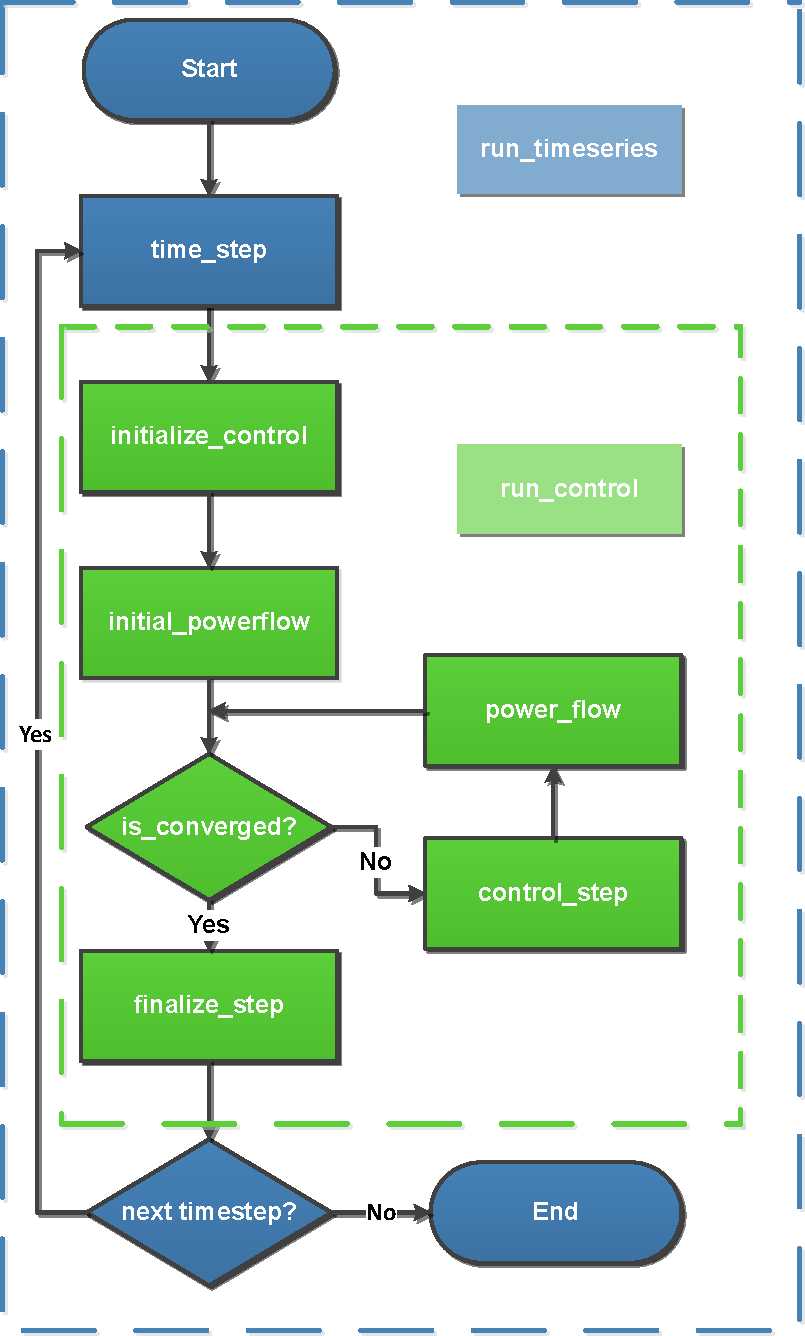
\includegraphics[width=0.32\linewidth]{timeseries_module_diag.pdf}
	\caption[\texttt{pandapower} times series module overview]{The diagram shows the timeseries loop of the timeseries module. The basic functionality is compute the power flow for each time step using the given values---such as sgens or loads. Step-wise convergence will depend on several factors, such as the network parameters (i.e. load magnitudes) as well as the algorithm used for solving the power flow problem. For more module details, see the \texttt{pandapower}  \href{https://pandapower.readthedocs.io/en/v2.10.1/timeseries/timeseries_loop.html}{wiki}.}
	\label{timeseries_module_diag}
\end{figure}
\FloatBarrier

The controller is a function whose purpose is to update the network values iteratively from a lookup table. The methodology will depend on your software of choice, but in our case we will be using the \texttt{pandapower} controllers made specifically for timeseries module. \Cref{timeseries_module_diag} shows a general overview of the built-in module. For our simulation, we will need 2 constant controllers for loads and sgens. Hereby, the correspondent data sources are the night dataframes that were defined in the DataAction class. Lastly, the timeseries iteration needs to be given a defined number of time steps, which in our case will be given by the index length of (either) night dataframe. With this information, the power flow can be computed iteratively based on tabular variable inputs. However, this will yield no useful results on its own, which is why we need to additionally define an output writer.

\paragraph{Time iteration and output:} An output writer is a function with a simple job of recording computed information, in an desired format, for each timeseries step. In our case, we will again be using the output writer function supplied with the \texttt{pandapower} timeseries module and outputting into an Excel file for the sake of convenience and troubleshooting. However, we aim to continue data processing in \texttt{pandas}, so we define another import function for said Excel results file. The imported dataframe can now provide relevant statistics and metrics. For our evaluation, the one of the key computations is the all-time minimum load value across all busses (see \cref{section_network_application} for more details).

\paragraph{Hosting capacity evaluation:} Hosting capacity was computed iteratively for a network in a single point in time. All pre-loaded network settings (even from the timeseries iteration) stay the same, except for the sgen columns---those need to be set to zero at first. Do not confuse the night sgen dataframe with the network sgen column; for a single point in time, only the network-defined sgens are taken into the calculation.

Iteration was performed over the list of sgen indices using a \texttt{for}-loop. The list is scrambled prior iteration in order to mimic uncoordinated charging patterns. An additional variable for storing the hosting capacity count is created. For each cycle of the loop, the following metric variables are computed by running a power flow calculation: minimum bus voltage magnitude per unit (vm p.u.) and maximum line loading percent. The next step is conditional. If the metric variables don't exceed preset limits, add an sgen value and increase the hosting capacity count by one. The loop proceeds onto the next cycle and computes the new power flow state of the network. Checking the metric variables again, if (at some point) the preset limits are exceeded, then we need to undo the effects of the last cycle. As such, the hosting capacity count is reduced by one and the last filled sgen is reset to zero. This breaks the loop. The function then computes one final power flow computation to obtain for an output plot and prints the maximum hosting capacity result.

\newpage
\subsection{Additional files}\label{subsection_additional}
In addition to the formally described python class file and jupyter data processing notebooks, several other files were used for the simulation project. They serve as an extension to the already discussed functionality and will therefore not be covered in similar detail but deserve mentioning nonetheless.

\paragraph{Bulk simulation:} Due to the random nature of the simulated load profiles selected from historical data, the results are prone to some degree of deviation. In particular, the network bus voltage minimum and maximum values in time are affected. While such deviations may not have a direct impact on the analysis of the hosting capacity evaluation, the two other scenarios---random charging time and energy community charging pattern---are more severely affected. Given the fact that our aim is to make a comparison between the random and the community scenarios, the simulation needed to be performed multiple times in order to obtain a reliable average and a convincing statement. For this purpose, a python file was created to perform bulk simulations. It follows through the same general steps described above with the inclusion of saving the vm p.u. minima (our limiting factor) to an external file per simulation per scenario. The loops are performed for 3 scenarios: random and community, as well as control, which does not include any active sgens. The results are loaded in and processed in jupyter and can be found in \cref{section_rand_vs_comm}.

\paragraph{Average minima and maxima times:} As supplementary part of the analysis, the time extrema for the entire dataset were calculated. The goal was to compute the time point of highest and lowest network bus loads. The computation was performed in jupyter and follows the same data parsing principles described earlier with the addition of a running average. This is required in order to analyze the general trend and not the outlying points; for this purpose, a rolling average of 10 minutes was found to give the best results. While this computation does not directly affect the core simulation, it does justify the chosen time window as well as the starting point of the energy community algorithm. See \cref{section_improvements} for how these two points can be used to improve the proposed model.

\newpage
\section{Network application}\label{section_network_application}
This section builds upon the fundamental operating principles of the two classes introduced in \cref{section_data_processing}. It aims to explain the usage of the python class file in order to obtain the three scenarios for the test feeder. First, consider the following assumptions.

The network used in the simulation is an altered version of the standard test feeder. The original network itself is 3-phase, which would require a different power flow model---in case of \texttt{pandapower}, that would be handled by \texttt{pandapower.pf.runpp\_3ph.runpp\_3ph()}. However, given the right circumstances, it is possible to treat a 3-phase network as single-phase; namely, if we assume that all network loads are balanced. This assumption is plausible and corresponds to most real-world households, to the extent that some power modeling software don't include a separate 3-phase computation option for this reason. With this assumption, all loads and sgens were defined and handled as single-phase in our simulation. The network was furthermore scaled down from 3-phase by dividing all the bus voltages by $\sqrt{3}$ to arrive at its single-phase equivalent.

The night-time bracket was chosen as \texttt{18:00:00--06:00:00} and serves as the allowed time frame for EV charging during the night. This night time is based around the common Western world business day hours, such as the standard office hours of 9 a.m. to 5 p.m. in USA; the time bracket is adjusted to account for often earlier starting hours in Europe. Hereby the EVs are assumed to be used for transportation to and from work, where charging is assumed to not be available. The chosen hours are commonly referred to as night time hours in this paper and code, even if the phrasing is applied somewhat generously.

One of the key factors of the simulation was the chosen sgen value. This corresponds to the charging rate of EVs, measured in kW. In terms of voltage levels---and by extension, the EV charging speed---AC charging is commonly separated into three levels. "The Levels 1 and 2 charging facilities can be installed in a private location while setting up of Level 3 charging facilities, involving separate wiring and transformer, requires permission from utility providers and are usually built in public charging stations" \cite{Das2020}. For this reason, level 2 charging was chosen. Most home charging stations that support level 2 charging usually provide an output of around 7\,kW. The most frequent figure on the market as of this writing appears to be 7.7\,kW, which was is why it was chosen as the sgen value.

With these assumptions and adjustments to the test feeder, the following 3 case scenarios were identified and analyzed.

\subsection{Critical case scenario}
This case scenario aims to address the hosting capacity of our test feeder given the most unfavorable circumstances. The evaluation process outline was as follows:
\begin{enumerate}
	\item Load and prepare dataset
	\item Create loads and sgens night dataframes
	\item Load and prepare test feeder network
	\item Define output writer and run the timeseries
	\item Import the voltage magnitude timeseries results
	\item Evaluate the all-time minimum and maximum load time points
	\item Load the network configuration for those time points
	\item Calculate hosting capacity at both critical time points
\end{enumerate}

Hereby, at step 8, the sgens are placed in a random network locations for two points (minutes) in time. Timeseries iteration in step 4 is used to locate those points in time, but it does not compute over any sgen values. The hosting capacity is expected to be under 100\,\% for this scenario.

\subsection{Random time scenario}
This case scenario aims to represent completely uncoordinated charging patterns over the night time window period. It's used as a comparison for the energy community scenario. The evaluation process is similar to the critical case scenario:
\begin{enumerate}
	\item Load and prepare dataset
	\item Create loads and sgens night dataframes
	\item Place sgens at random locations in the network
	\item Load and prepare test feeder network
	\item Define output writer and run the timeseries
	\item Import the voltage magnitude timeseries results
	\item Evaluate the all-time minimum load time point
	\item[Opt:] Load network configuration for all-time minimum vm p.u. time point
\end{enumerate}

The main difference from the critical case scenario is that we load sgens in our network before we run the timeseries iteration. Since the sgens charging times are spread across the night window, all sgens can be active at one point or another. This only becomes problematic should a relatively large number of sgens happen to be charging at once. At the same time, the household load profiles may offset a potential network overload if the charging convergence happens late a night when the loads are lowest---since most people are asleep and little to no household appliances are running.


\subsection{Energy community scenario}
This case scenario aims to propose the concept of semi-coordinated charging, whose main idea is that of simplicity with minimum requirements. As mentioned in  \cref{section_literature_review}, there is no shortage of highly optimized models proposed. Both centralized charging management algorithms and decentralized/distributed charging mechanisms should undoubtedly serve as the goal of EV technology and its future implementation. That being said, these models remain mostly conceptual in nature, owing to their intricacy of operation as well as high upfront resource demands.

While there have been tremendous advancements made in making individual grid elements and devices smarter, there's yet to exist a truly unified system at scale. The internet of things (IoT) offers a glimpse into a fully synchronized smart-device architecture but this concept does not transfer to vehicles as readily, due to their mobile nature and dependence on existing infrastructure. Arguably the minimum precondition for large-scale smart EV charging mechanisms is the existence of installed smart meters in residential homes. The spread of smart meter technology has proven to be highly incentivised by progressive energy tariffs and some success has been found in countries across Europe, such as Spain adopting a Real-Time-Pricing (RTP) tariff in 2015. Unfortunately, many countries are still lagging behind the practically-feasible due to their complex governmental policies---Germany in particular has been struggling with residential smart meter roll out, despite its ambitious push towards embracing renewables. Needless to say, there still remain plenty of obstacles in the way of widespread, advanced EV charging systems.

With these considerations in mind, this paper proposes the most simplistic way to improve grid stability through altered charging patterns. This method does not rely on the existence of smart meters or intelligent controllers and can therefore be implemented in any local network (section) in a form of a rudimentary energy community. In the scope of this paper, the concept of energy community is also simplified to its most basic premise---coordinated energy use. As such, the method can be viewed as the first stepping-stone in transition towards smart grid EV charging. 

\subsubsection{Theoretical considerations}\label{subsubsection_theoretical_con}

Consider the following theoretical network depicted in \cref{comm_topology}, not dissimilar from the original test case network.

\begin{figure}[htpb]
	\centering
	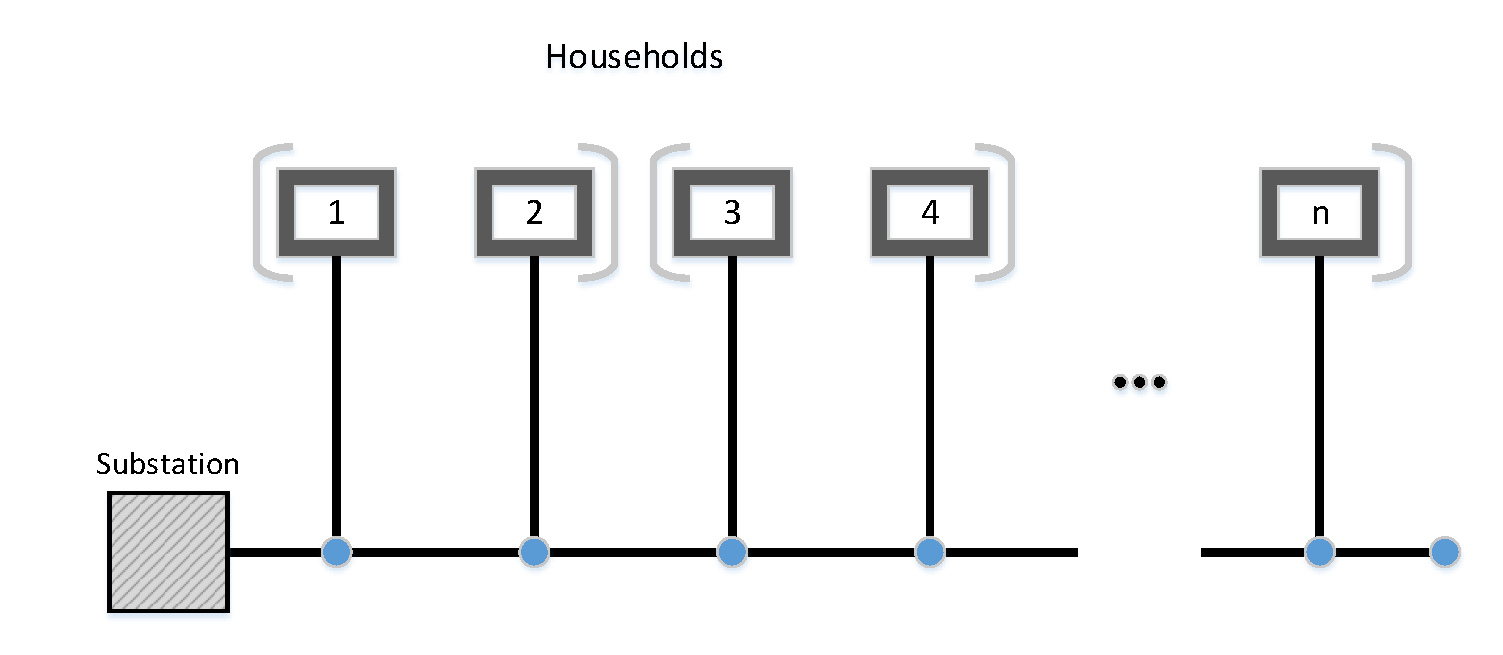
\includegraphics[width=0.7\linewidth]{comm_topology}
	\caption[Theoretical energy community network scenario]{A theoretical network scenario for linearly placed single-line households. The energy community aims to include every new household member.}
	\label{comm_topology}
\end{figure}


The linear topology of the theoretical network is reminiscent of the test feeder. Known as radial operation, this is the most widespread design in both medium-voltage (MV) and low-voltage (LV) networks. Hereby, the North American system differs from the European in transformer placement and is not discussed further, as the application of the developed model is aimed at the European LV grid, although the results can in some extent be transferable. Furthermore, spot networks (commonly found in business and industry districts) as well as grid networks (typical for downtowns of large cities) are omitted in this theoretical scenario.

The theoretical radial network demonstrates a relatively straightforward load pattern. Every consecutively added household down the line from the substation increases the overall network load; the last household $n$ acquires the network minimum in voltage magnitude in case of constant household load profiles. The goal is then to avoid the critical case scenario of network overload, which is most likely to happen at, or close to, the $n$'th household bus. Given these spacial considerations, we must also distribute the sgen loads temporally so as to minimize the network load. This amounts to two conditions. First, avoid multiple sgens charging at the same time as much as possible---this is the deciding factor between the two conditions. The best case scenario (generally) is an even distribution of sgens in time. Second, should there be a crossover in charging times, the beginning of the network line should be prioritized, since its local voltage magnitudes will be (albeit slightly) lower than those at the end of the transmission line. The crossover of charging times is guaranteed to occur for a sufficiently large $n$ and depends on charging time, which we assume is constant across all households. Next, consider the concept of coordination.

Coordination of energy use, in the context of our energy communities, begins with communication between multiple parties. In the most primitive sense, this can be as simple as an agreement between two neighbors to not charge their EVs at the same time of day. Assuming they both come home from work around the same time and want to immediately plug in their EVs to charge, one neighbor can agree to start charging after the other one is done. This alone will have an obvious beneficial effect on grid stability but would still imply most households charging around peak grid hours in the evening. The more coordinating pairs, the better. Eventually, we can extend this idea to the entire neighborhood, thus forming an energy community. The community decides to agree on dedicated charging times for individual households based on the philosophy described above.

Referring back to \cref{comm_topology}, the energy community decides to allocate charging times iteratively, starting from the household closest to the substation. The first household will take the charging time closest to peak grid hours in the evening, the second will take the next available time slot after the first and so on. Once all available charging time slots per night have been filled, the time slots will cycle times (the same way they were initially filled) for new sgens.

\subsubsection{Test feeder application}
In the case of the test feeder, the allocated sgen charging times and cycles can be seen in \cref{sgen_comm_times}. On average we can expect $55\, \text{sgens} / 12\, \text{hours} \approx 4.583$ sgens per given hour in the night frame, which correlates with our results.

\begin{table}[htpb]
	\centering
	\begin{tabular}{c c c}
		\toprule
		start time & end time & sgens active \\
		\midrule
		\texttt{18:00:00} & \texttt{18:59:00} & 5\\
		\texttt{19:00:00} & \texttt{19:59:00} & 5\\
		\texttt{20:00:00} & \texttt{20:59:00} & 5\\
		\texttt{21:00:00} & \texttt{21:59:00} & 5\\
		\texttt{22:00:00} & \texttt{22:59:00} & 5\\
		\texttt{23:00:00} & \texttt{23:59:00} & 5\\
		\texttt{00:00:00} & \texttt{00:59:00} & 5\\
		\texttt{01:00:00} & \texttt{01:59:00} & 4\\
		\texttt{02:00:00} & \texttt{02:59:00} & 4\\
		\texttt{03:00:00} & \texttt{03:59:00} & 4\\
		\texttt{04:00:00} & \texttt{04:59:00} & 4\\
		\texttt{05:00:00} & \texttt{05:59:00} & 4\\
		\bottomrule
	\end{tabular}
	\caption[Energy community charging times for test feeder network]{Energy community charging times for test feeder network.}
	\label{sgen_comm_times}
\end{table}

For spacial allocation, the sequence of predefined sgen locations in \texttt{pandapower} test feeder network was used. Additionally, line loading is generally expected to be around 1\% per household line and was shown not to be the limiting factor for hosting capacity calculation.


\chapter{Results and Discussion}
The simulation results can be divided into two groups: hosting capacity and random vs energy community scenarios comparison. The hosting capacity results feature single simulation examples chosen at random. The random vs energy community scenarios comparison results are based on a set of simulations and consequent group averages.

\section{Hosting capacity}
Hosting capacity calculations began by computing the timeseries with no sgens active. The network bus load example results can be seen in \cref{hosting_time_series_table}. As expected, the the voltage magnitude per unit drops with each bus load---hereby the extrema are sometimes shared across multiple busses (even at higher significant figure counts). The time points for voltage magnitude extremes are unique however, which leads to two cases: minimum bus vm p.u and maximum bus vm p.u.

\begin{table}[htpb]
	\centering
	\begin{tabular}{lrrrlrrr}
		\toprule
		& bus\_0 & bus\_1 & bus\_2 & \dots & bus\_904 & bus\_905 & bus\_906 \\
		\midrule
		count & 721.000 & 721.000 & 721.000 & \dots & 721.000 & 721.000 & 721.000 \\
		mean & 1.050 & 1.050 & 1.049 & \dots & 1.031 & 1.031 & 1.031 \\
		std & 0.000 & 0.000 & 0.000 & \dots & 0.006 & 0.006 & 0.006 \\
		min & 1.050 & 1.049 & 1.049 & \dots & 1.014 & 1.014 & 1.014 \\
		25\% & 1.050 & 1.050 & 1.049 & \dots & 1.027 & 1.027 & 1.027 \\
		50\% & 1.050 & 1.050 & 1.050 & \dots & 1.033 & 1.033 & 1.033 \\
		75\% & 1.050 & 1.050 & 1.050 & \dots & 1.036 & 1.036 & 1.036 \\
		max & 1.050 & 1.050 & 1.050 & \dots & 1.041 & 1.041 & 1.041 \\
		\bottomrule
	\end{tabular}
	\caption[Example simulation timeseries results]{Example simulation timeseries results. The first bus's vm p.u. is at the upper acceptable bracket limit (both minima and maxima), whereby the last bus's vm p.u. minima is close to the middle of the bracket, which is optimal. This indicates that historical network loads are well suited for this network.}
	\label{hosting_time_series_table}
\end{table}

The network graphs for hosting capacity time extremes calculation are shown in \cref{hopsting_cap_figures}. Visually, we can see a big difference in color profiles for cases with different starting time points. \Cref{hopsting_cap_figures_a} shows significant line stress in the bottom two branches of the network (seen in yellow), as opposed to \cref{hopsting_cap_figures_c} where the entire network is stabilized, implying less deviation between bus loads. Hereby we expect a greater hosting capacity for the maximum bus voltage time point case due to its color profile homogeneity (shown in red) and a bigger maximum range of vm p.u., which would allow to accommodate more sgens at the lower branches. As far as filled sgen hosting capacity graphs are concerned, there's little visual difference between \cref{hopsting_cap_figures_b} and \cref{hopsting_cap_figures_d} at this scale. For more insight, consider numerical data in \cref{extremes_summary} and \cref{hosting_cap_stats}.

\FloatBarrier
\begin{figure*}
	\centering
	\begin{subfigure}[b]{0.475\textwidth}
		\centering
		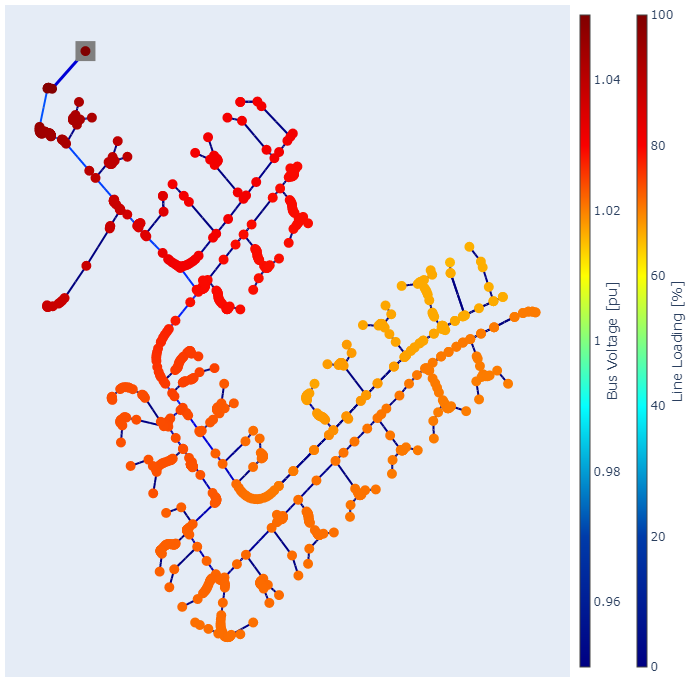
\includegraphics[width=\textwidth]{hosting_cap_min_empty}
		\caption[]
		{{\small No sgens at min bus voltage}}    
		\label{hopsting_cap_figures_a}
	\end{subfigure}
	\hfill
	\begin{subfigure}[b]{0.475\textwidth}  
		\centering 
		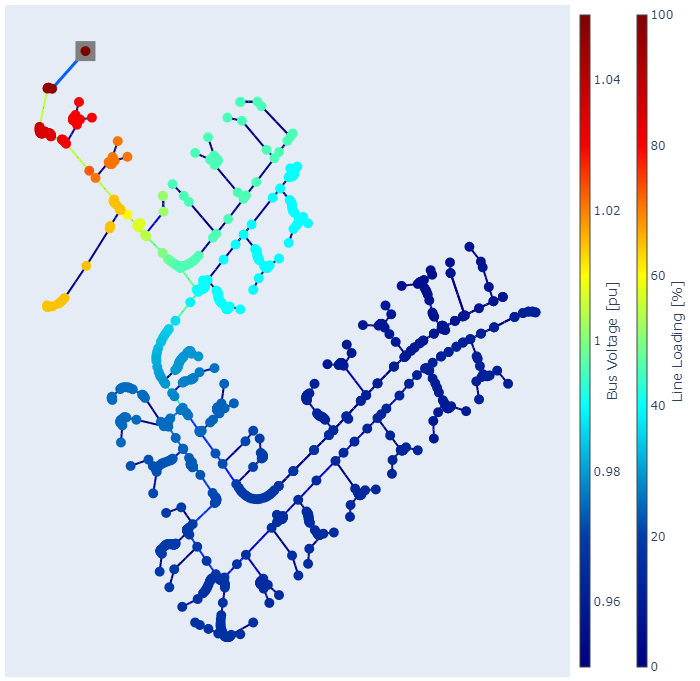
\includegraphics[width=\textwidth]{hosting_cap_min_full}
		\caption[]
		{{\small Filled sgens at min bus voltage}}    
		\label{hopsting_cap_figures_b}
	\end{subfigure}
	\vskip\baselineskip
	\begin{subfigure}[b]{0.475\textwidth}   
		\centering 
		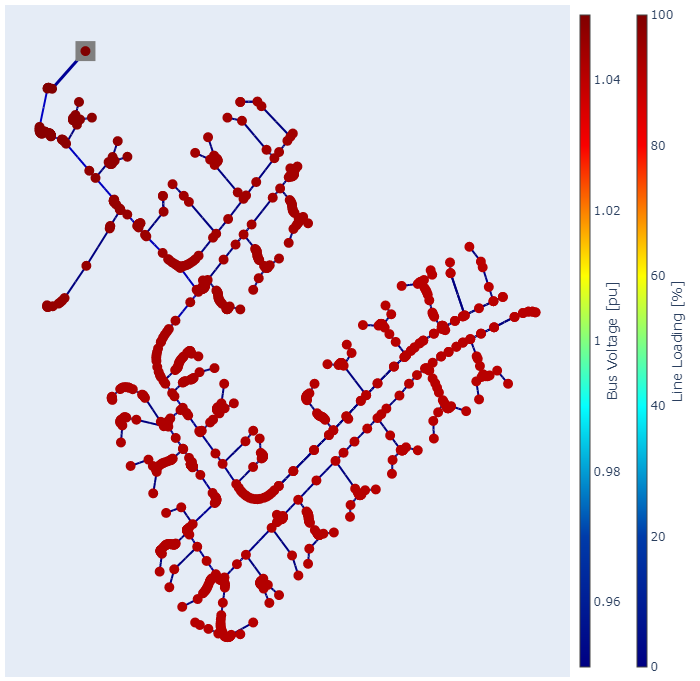
\includegraphics[width=\textwidth]{hosting_cap_max_empty}
		\caption[]
		{{\small No sgens at max bus voltage}}    
		\label{hopsting_cap_figures_c}
	\end{subfigure}
	\hfill
	\begin{subfigure}[b]{0.475\textwidth}   
		\centering 
		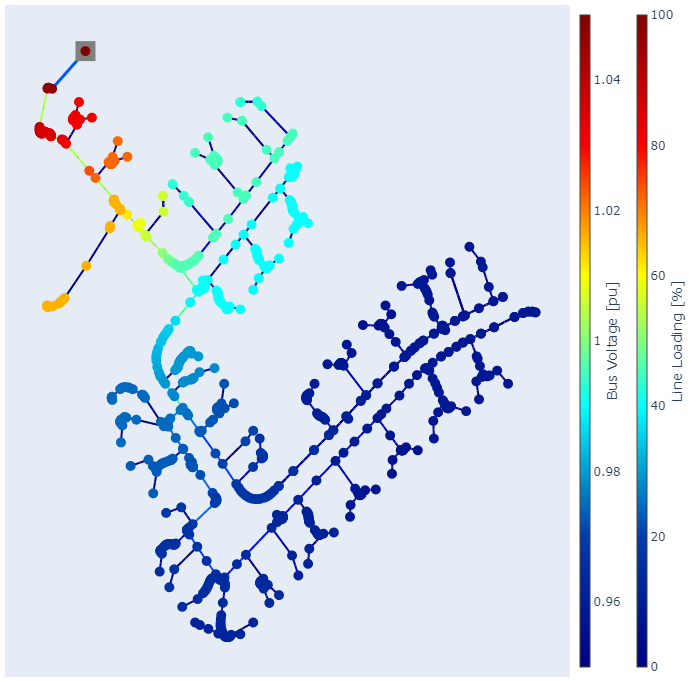
\includegraphics[width=\textwidth]{hosting_cap_max_full}
		\caption[]
		{{\small Filled sgens at max bus voltage}}    
		\label{hopsting_cap_figures_d}
	\end{subfigure}
	\caption[Comparison of hosting capacities for time extremes]
	{\small Comparison between hosting capacity during minimum (subfigures (a) and (b)) and maximum (subfigures (c) and (d)) load time cases with and without sgens.} 
	\label{hopsting_cap_figures}
\end{figure*}
\FloatBarrier

The details of time point cases for each network are shown in \cref{extremes_summary}. We can see a significant difference in minimum vm p.u. values between the "Min bus empty" and "Max bus empty" cases. This is a numerical indication of a greater hosting capacity potential for the maximum time point case. For the columns "Min bus full" and "Max bus full", we observe no significant difference between the two min values---this indicates that the maximum hosting capacity has been reached in both cases at a vm p.u. lower bracket.

\begin{table}[htpb]
	\centering
	\begin{tabular}{lcccc}
		\toprule
		& Min bus empty & Min bus full & Max bus empty & Max bus full \\
		\midrule
		count & 907.000 & 907.000 & 907.000 & 907.000 \\
		mean & 1.020 & 0.980 & 1.042 & 0.976 \\
		std & 0.009 & 0.022 & 0.002 & 0.021 \\
		min & 1.005 & 0.953 & 1.039 & 0.950 \\
		25\% & 1.014 & 0.963 & 1.040 & 0.963 \\
		50\% & 1.018 & 0.975 & 1.041 & 0.970 \\
		75\% & 1.025 & 0.994 & 1.043 & 0.987 \\
		max & 1.050 & 1.050 & 1.050 & 1.050 \\
		\bottomrule
	\end{tabular}
	\caption[Hosting capacity voltage magnitudes in detail]{Hosting capacity voltage magnitudes in detail.}
	\label{extremes_summary}
\end{table}

The key results of the hosting capacity simulations are summarized in \cref{hosting_cap_stats}.

\begin{table}[htpb]
	\centering
	\begin{tabular}{lcc}
		\toprule
		& Minimum bus voltage & Maximum bus voltage \\
		\midrule
		number of sgens & 6 & 12 \\
		total capacity [\%] & 10.9 & 21.8 \\
		\bottomrule
	\end{tabular}
	\caption[Hosting capacity results]{Hosting capacity results.}
	\label{hosting_cap_stats}
\end{table}

The scenario results show a rather low hosting capacity for both time point cases. As expected, the best case of maximum bus voltage has a significantly better hosting capacity---about double that of the worst case of minimum bus voltage. In a way, this is alarming because the probability of a network overload is definitely not negligible: it only takes $\approx10\,\%$ of all households to charge their EVs during peak hours to cause a potential brownout/blackout. Furthermore, this time point is the most probable charging time point for any given individual under our assumptions of European work hours; without the presence of smart meters, a person is most likely to park their EV and set it to charge immediately. Considering the habitual nature of human actions, a network overload is only a matter of time in this case.

That being said, the issue can be easily avoided with relatively little intervention. Undoubtedly, all EV chargers do (and if not, will soon) include a time setting option, which is very easy to implement. Hereby, an EV owner only needs to enable and setup the charging hour parameter once, which is a matter of seconds. At the same time, one cannot deny that not everyone will bother to do so, nor that any potential software/firmware updates will reset the setting. As such, one is able to compensate for technological shortcomings (i.e. lack of smart EV charging) with conscious human intervention (i.e. manually setting the EV to charge outside of peak hours) and vice versa.

With this discussion we arrive at the transitional phase of semi-smart charging and the comparison between uncoordinated and semi-coordinated scenarios.


\section{Random vs energy community comparison}\label{section_rand_vs_comm}
This section puts the energy community algorithm to the test against a random charging pattern. A representative graphical result is shown in \cref{random_vs_en_comm}.

\FloatBarrier
\begin{figure*}[htpb]
	\centering
	\begin{subfigure}[b]{0.475\textwidth}
		\centering
		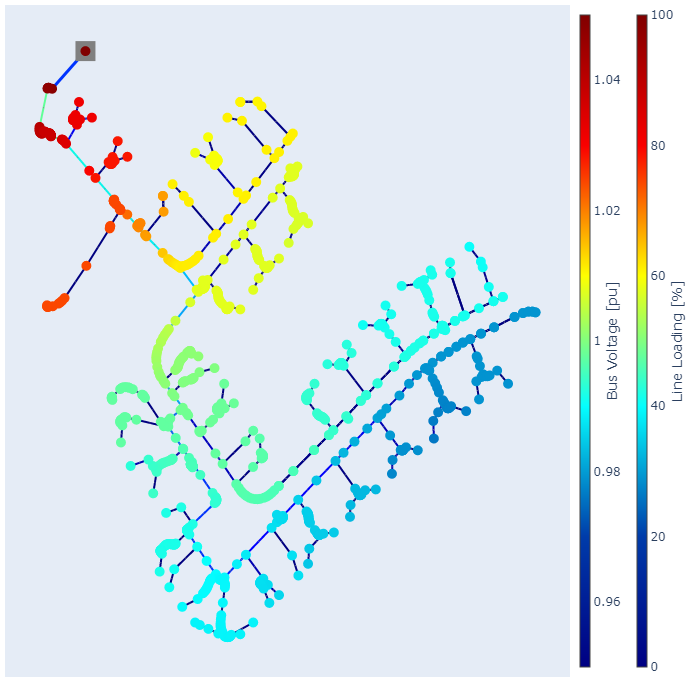
\includegraphics[width=\textwidth]{random_loads_min_full}
		\caption[]
		{{\small Random scenario}}    
		\label{random_vs_en_comm_a}
	\end{subfigure}
	\hfill
	\begin{subfigure}[b]{0.475\textwidth}  
		\centering 
		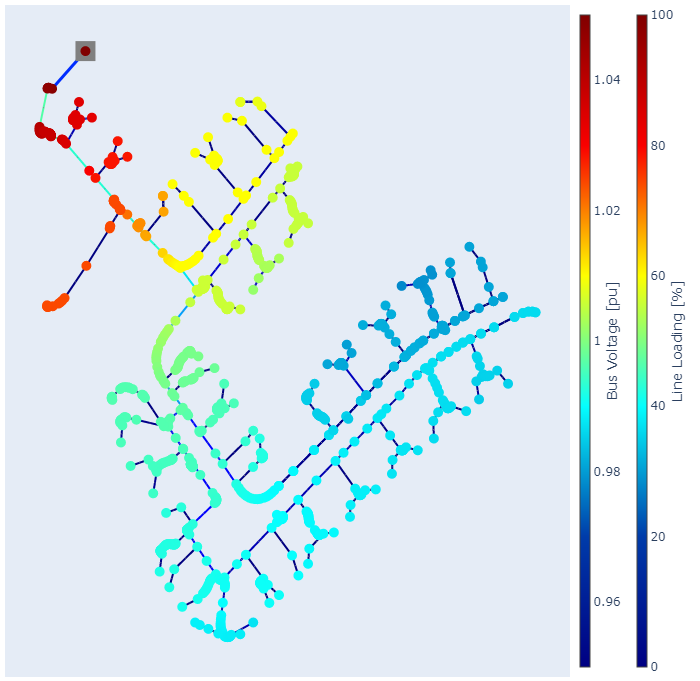
\includegraphics[width=\textwidth]{en_comm_min_full}
		\caption[]
		{{\small Energy community scenario}}    
		\label{random_vs_en_comm_b}
	\end{subfigure}
	\caption[Comparison of hosting capacities for random and energy community scenarios]
	{\small Graphical comparison between random and energy community scenarios. These are two random example simulations.} 
	\label{random_vs_en_comm}
\end{figure*}
\FloatBarrier

The random scenario represents an uncoordinated charging pattern with all 55 households charging at some point during the night window. While the spacio-temporal allocation of sgens is random, we can expect results generally similar to those shown in \cref{random_vs_en_comm_a}. A defining characteristic of this scenario is the local maximum line load on the lowest branch (seen in darker blue). This corresponds with our theoretical network model characteristic in \cref{subsubsection_theoretical_con} and outlines one of the biggest weaknesses of radial operation topology. It is reassuring to then see a visual improvement in this area in \cref{random_vs_en_comm_b}. The lower branch load has a considerably more even color gradient indicating a more even distribution of loads at a lower voltage magnitude. Interestingly, the local minimum for the energy community scenario is located on a different branch to that of the random community scenario, slightly higher up the sgen list (closer towards the substation). Even then, that upper branch is still showing a lower bus voltage throughout in comparison to the random scenario's lower branch.

\begin{table}[htpb]
	\centering
	\begin{tabular}{lccc}
		\toprule
		Scenario & Random & Community & Control \\
		\midrule
		simulations count & 100 & 100 & 100 \\
		avg min voltage mag [p.u.] & 0.941 & 0.971 & 1.010 \\
		bracket deviation [\%] & 108.6 & 79.2 & 40.3 \\
		\bottomrule
	\end{tabular}
	\caption[Comparison between random and energy community scenarios]{Comparison between random and energy community scenarios.}
	\label{table_random_vs_comm}
\end{table}

To obtain a more concrete set of results, bulk simulation was performed. The results are summarized in \cref{table_random_vs_comm}. The raw data gives us the average minimum vm p.u. for both random and energy community scenarios; an additional control scenario represents a test feeder with no sgens active for comparison. Notably, the random charging pattern on average leads to a network overload (0.941 vm p.u.), whereas the energy community scenario doesn't (0.971 vm p.u.). The control value falls within 1\% of the optimal network bus load value, indicating a good choice of parameters. Total simulation runtime for 3 scenarios, 100 runs each, was 3 hours and 40 minutes (with no hardware bottleneck).

The results are additionally interpreted via the so-called bracket deviation metric in this paper. Recall that the load bracket is defined as the acceptable range of bus voltage magnitude per unit. Following common network guidelines, it's taken as the open interval $(0.95\,, 1.05)$. Load bracket deviation percent hereby is defined as:

\begin{equation}
	\text{Deviation [\%]} = \frac{\text{upper bracket} - \text{average voltage}}{\text{upper bracket}-\text{lower bracket}}\times 100
\end{equation}

Taking the difference of two brackets, we can show that the energy community scenario is approximately 29.4\% more effective than random charging scenario on average. This was a pleasantly surprising result, given how rudimentary and overly-simplified the energy community algorithm is. The next section will further explain the simulations' shortcomings and suggest various improvements.


\chapter{Conclusion}\label{section_improvements}
This paper presents several key findings on the topic of EV integration. Firstly, the hosting capacity of a typical European low-voltage grid is surprisingly low ($\approx10\,\%$) for a worst-case scenario. This serves as a strong motivation for further research and investment required in the topic of grid stability. Secondly, this paper introduces a simple but relatively effective spacio-temporal algorithm for EV charging. The semi-coordinated charging algorithm was proven to be more effective ($\approx30\,\%$) than the uncoordinated charging scenario, which is surprisingly good given its extreme simplicity. One can argue in favor of unoptimized algorithms when taking into account the public's perception of energy transparency. An algorithm such as this one could prove to be a valuable stepping-stone for the purposes of transition towards the future of smart grids and EV integration. Additionally, consider the following limitations of this paper's work.

Perhaps the biggest uncertainty in the simulation parameters was the charging window. Ideally, the charging window should represent the average charging time for a single household under the most common circumstances. If one were to calculate said average from real-world statistics, one would have to consider (at least) the following average values: daily driving distance, daily time spent in traffic, typical EV energy consumption/efficiency and typical battery discharge rate. This paper assumes that the end user will continuously top-up the EV battery on a daily basis. Hereby, the EV battery technology is the key factor to widespread EV adoption. The field is rapidly developing, which makes it hard to predict precise technical details, such as maximum charging rates. At the same time, since it is highly unlikely to expect Level 3 DC charging reach widespread household integration, our assumption for 7.7\,kW charging rate remains plausible. Workplace or public charging stations are most likely to see installation in the near future, which could reduce the total number of household EV charging stations drastically. Lastly, a completely thorough analysis could additionally factor in energy tariffs and their effects on person's charging habits.

The energy community spatio-temporal algorithm is in no way optimal and is an extreme over-simplification of the problem. Its main purpose is to serve as a starting point for when there is none, and to serve as a demonstration for what minimum effort can achieve in the context of grid stability. Consider the shortcomings of both dimensions separately:

\paragraph{Spacial:} The current algorithm relies on correct ordering of busses for iteration and does not account for significant deviation or branching from linear topology. This implies that the results depend significantly on manual ordering of busses, which can become unintuitive with enough complexity. A possible solution would be to implement a tree path length comparison algorithm, though certain cases such as branches of equal lengths may be difficult to account for. (This is even possible to do in \texttt{pandapower} using \texttt{calc\_distance\_to\_bus()} function.) Alternatively, one could limit the current algorithm to smaller sections of the network and run it locally, since it would still optimize for distance from substation. As last resort, constrained brute-forcing different bus ordering cases should not take long, given the relative simplicity of the simulation.

\paragraph{Temporal:} There are two time-based shortcomings of the algorithm. Firstly, the programmed value for sgen allocation starting time (\texttt{18:00:00}) does not match the computed historical dataset peak-time (\texttt{19:23:00}) as dictated in \cref{subsubsection_theoretical_con}. A function for proper sgen charging time was actually written, which involved nested time-conditional \texttt{for}-loops. However the updated function was eventually discarded due to the complexity of new code, as the energy community function would also need to be rewritten and there was simply not enough time.

Secondly, average sgen distribution in time is not optimal. Ideally, most sgens would be shifted towards the time of vm p.u. minimum, which was computed to be \texttt{02:26:00} based on historical data. Referring back to \cref{sgen_comm_times}, we can see that there are 5 sgens active during the \texttt{18:00:00}--\texttt{00:00:00} interval, followed by the remaining time slots at night to be filled with 4 sgens---this ordering should be reversed. Unfortunately there is no easy fix that comes to mind, since it would require one to separate the spacial from the temporal, thus writing a new algorithm altogether. What this simulation ultimately shows however, is that the spacial component has a far greater impact on the results than the temporal and that this shortcoming could therefore be ignored.

A considerable amount of effort was put into making the data analysis code "proper" (to the best of author's knowledge and ability at the time). Nevertheless, several problems remained unfixed: these should not have had a negative impact on the simulation results, only on the runtime. For instance, the dataframe list splitting function ultimately discards 2 days of data per list (beginning and end). In scope of the total size of the household dataset, this is a negligible loss of information but it could still use improvement. Alternatively, one could make use of additional residential household datasets from the Open Power System Data.

A more problematic issue was the following terminal dual warning:
\noindent
\begin{itemize}[leftmargin=2.1cm]
	\item[\texttt{pandapower}] create\_jacobian.py:\\
	\texttt{"RuntimeWarning: invalid value encountered in true\_divide}"
	\item[\texttt{scipy}] linsolve.py:\\
	\texttt{"MatrixRankWarning: Matrix is exactly singular"}
\end{itemize}
This would only appear occasionally, seemingly independent of most simulation parameters (such as load magnitudes or sgen values). It did not prevent the power flow from returning a solution and the results always appeared within the expected range. As such, this warning was mostly avoided through re-runs or, in case of the bulk simulation, through averaging of results. Lastly, occasionally there appeared to be mismatch in index and table lengths when parsing the dataframe tables, which would be solved via a simple rerun. It's possible that this bug is kernel-related to the local python installation; like the others above-mentioned, it does not impact the validity of results.

\bibliographystyle{IEEEtran} %displays URLs
\bibliography{bib_library}
\addcontentsline{toc}{chapter}{Bibliography}

\chapter*{Appendix}\label{chapter_appendix}
\addcontentsline{toc}{chapter}{Appendix}

\lstinputlisting[language=Python]{"C:/Users/panto/Documents/git/personal/EV_energy_comm/python/data_process.py"}

\end{document}

%------------------------------------------------------------------

%\FloatBarrier
%\begin{figure}[htpb]
%	\centering
%	\includegraphics[width=0.9\linewidth]{blah}
%	\caption{blah}
%	\label{blah}
%\end{figure}
%\FloatBarrier